\mode*

\mode<all>{\input{../hash-review.tex}}


% XXX review the approach to bitcoin, perhaps start in the other end?
\section{Cryptocurrencies}

Bitcoin is a decentralized cryptocurrency proposal by \textcite{Nakamoto2008bap}.

\ltnote{%
  \textbf{Object of learning}: How Bitcoin combines public logs, hash chaining,
  proof-of-work, and Merkle trees to obtain ordering and decentralized
  agreement.

  \textbf{Try-first}: We will repeatedly ask what can go wrong before
  introducing the mechanism that fixes it.
}

\begin{frame}
  \begin{idea}[Bitcoin~\cite{Nakamoto2008bap}]
    \only<presentation>{%
      \begin{itemize}
        \item Decentralized: no central authority.
        \item All transactions are in a public log.
        \item \emph{Sort of} democratized: uses majority consensus.
      \end{itemize}
    }
    \only<article>{%
      Bitcoin replaces a central authority with a peer-to-peer network.
      Transactions are recorded in a public log, and nodes accept the history
      with the most accumulated proof-of-work as the \,\enquote{best}\, history.
    }
  \end{idea}
\end{frame}

%\begin{frame}
%  \begin{idea}
%    \begin{itemize}
%      \item Nya bitcoins skapas kontinuerligt med konstant avtagande hastighet.
%      \item Ett bitcoins kan delas i godtyckligt antal delar, och delar kan sedan 
%        sättas ihop till större delar.
%      \item Överföringar är permanenta.
%      \item Låga överföringsavgifter.
%    \end{itemize}
%  \end{idea}
%\end{frame}

\subsection{A transaction is money}

\begin{frame}
  \begin{figure}
    \includegraphics[width=0.7\textwidth]{fig/bitcoin-transfer.png}
    \caption{Transfer from Owner 1 to Owner 2 to Owner 3.
    Image:~\cite{Nakamoto2008bap}.}
  \end{figure}

  \pause

  \begin{idea}
    \only<presentation>{%
      \begin{itemize}
        \item \enquote{Money} is represented by transactions.
        \item Ownership is a chain of signatures.
      \end{itemize}
    }
    \only<article>{%
      In Bitcoin, there is no separate \,\enquote{coin object}. Instead, the
      thing that is transferred is a \emph{transaction} that references a
      previous transaction and authorizes a new owner. In that sense,
      \enquote{a transaction is money}.
    }
  \end{idea}
\end{frame}

\ltnote{%
  \textbf{Variation pattern}: Generalization from everyday \enquote{money} to a
  formal representation.

  \textbf{Critical aspects}: There is no separate coin object; what circulates
  is an authenticated ownership record (a chain of signatures).
}

%\begin{frame}
%  \begin{figure}
%    \includegraphics[width=0.4\textwidth]{fig/bitcoin-transaction.png}
%    \caption{A transaction.
%    Image:~\cite{Nakamoto2008bap}.}
%  \end{figure}
%\end{frame}

\subsection{Problems}

\begin{frame}
  \begin{question}
    \only<presentation>{%
      \begin{itemize}
        \item What is the main problem to solve: distribution or agreement?
        \item What can a malicious node do during distribution?
      \end{itemize}
    }
    \only<article>{%
      Before we introduce hashing, chaining, and proof-of-work, we should be
      explicit about what the network setting breaks. Simply broadcasting
      transactions is not enough: nodes may receive different subsets (or receive
      them in different orders), and an adversary can selectively relay or delay
      information.
    }
  \end{question}
\end{frame}

\begin{frame}
  \begin{figure}
    \includegraphics[height=0.8\textheight]{fig/distribute-tx.pdf}
    \caption{Distributing transactions}
  \end{figure}

  \vfill

  \only<presentation>{%
    \begin{remark}
      \begin{itemize}
        \item Broadcasting is easy; consistency is not.
      \end{itemize}
    \end{remark}
  }
  \only<article>{%
    \begin{remark}
      Broadcasting helps disseminate transactions, but it does not create a
      single agreed-upon history.
    \end{remark}
  }
\end{frame}

\begin{frame}
  \begin{figure}
    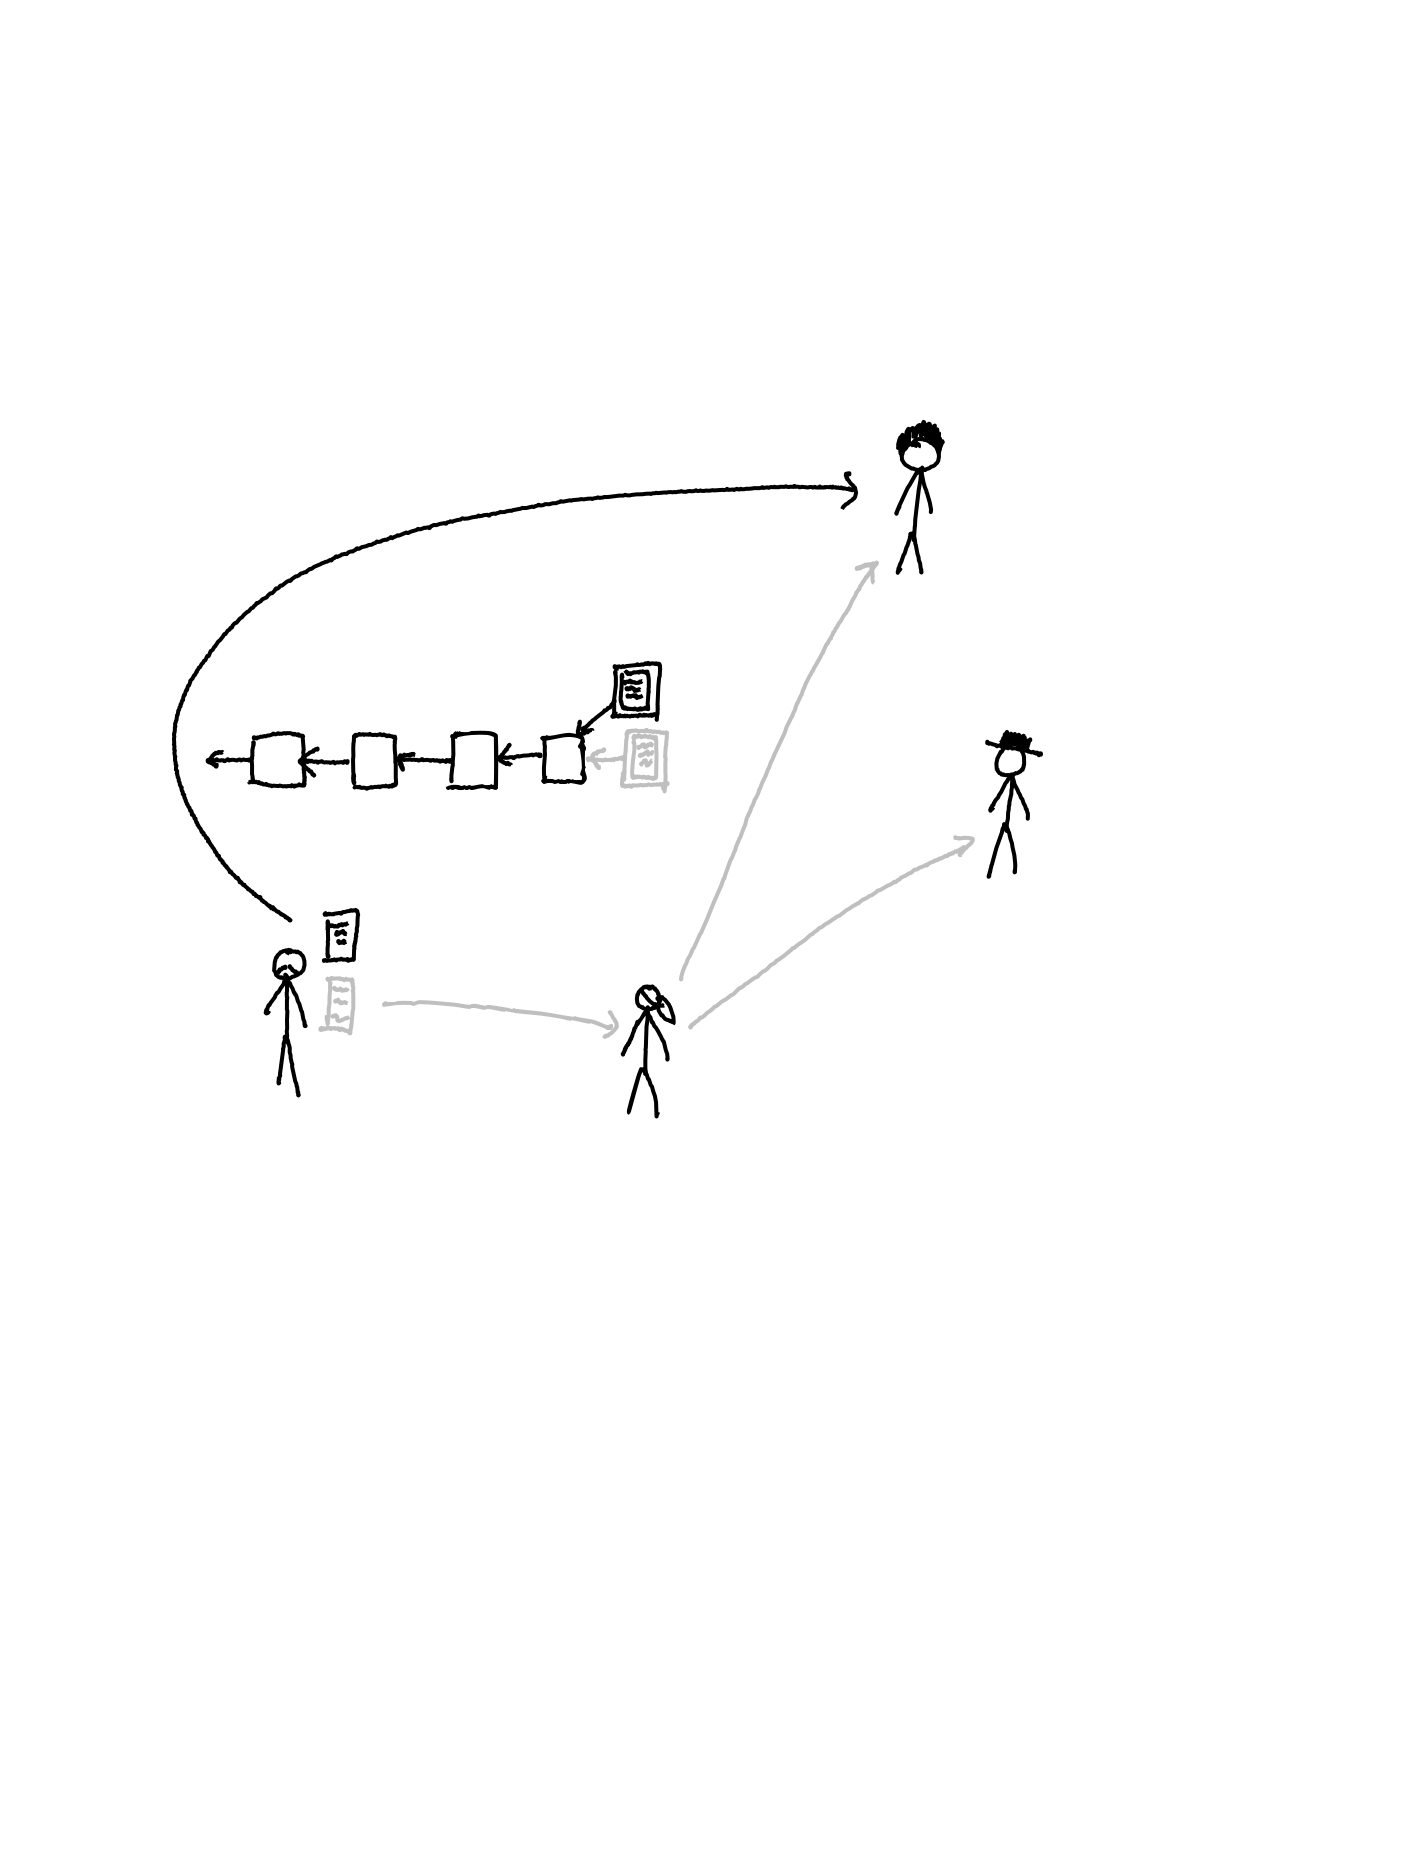
\includegraphics[height=0.8\textheight]{fig/distribute-tx-malicious.pdf}
    \caption{Maliciously distributing transactions}
  \end{figure}

  \vfill

  \begin{question}
    \only<presentation>{%
      \begin{itemize}
        \item If I can relay different messages to different nodes, what breaks?
      \end{itemize}
    }
    \only<article>{%
      If a malicious party can influence message propagation, different nodes may
      end up with different views of \,\enquote{the current state}. This makes
      double spending possible even if each transaction is individually signed.
    }
  \end{question}
\end{frame}

\begin{frame}
  \begin{figure}
    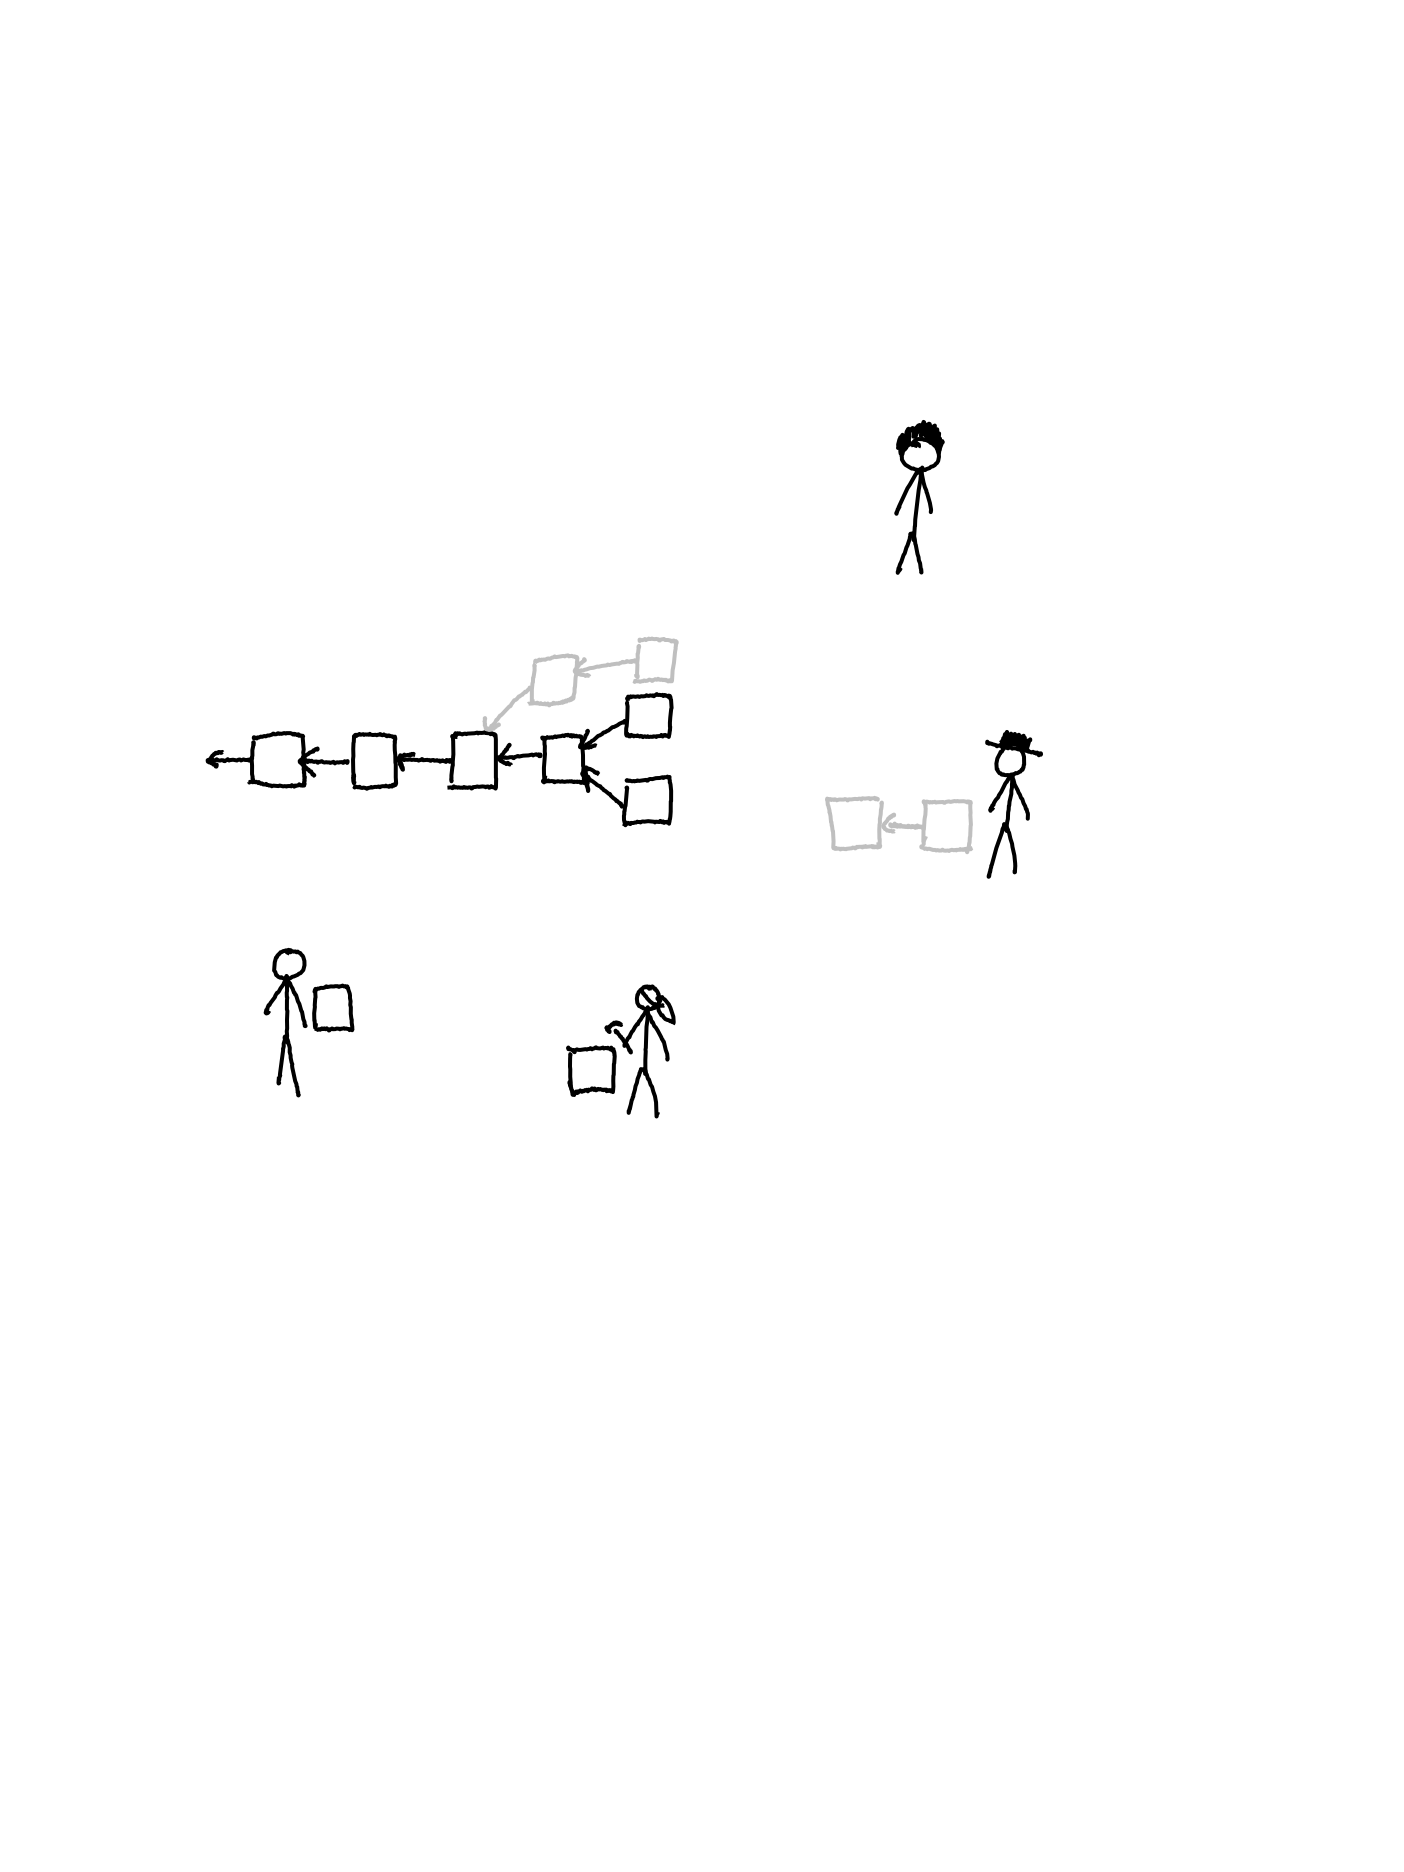
\includegraphics[height=0.8\textheight]{fig/mining.pdf}
    \caption{How a block chain is agreed upon.}
  \end{figure}

  \vfill

  \begin{question}
    \only<presentation>{%
      \begin{itemize}
        \item What is the network actually \,\enquote{agreeing on}? A set or an order?
      \end{itemize}
    }
    \only<article>{%
      The protocol must not only spread transactions but also produce a public,
      verifiable \,\emph{ordering}\, of them. Proof-of-work is the mechanism that
      makes one proposed ordering more credible than another.
    }
  \end{question}
\end{frame}

\ltnote{%
  \textbf{Try-first}: Start with failure modes in a network setting before
  naming the mechanisms (hash chaining, proof-of-work).

  \textbf{Variation pattern}: Contrast between (i) dissemination of information
  and (ii) shared agreement on an ordering.

  \textbf{Critical aspects}: Signatures give authorization, but not a global
  order or consensus under delayed/selective communication.
}

%\begin{frame}
%  \begin{idea}[Piecing together all ideas]
%    \begin{itemize}
%      \item Every transaction is distributed to all participating nodes.
%      \item Each node collects transactions into a block.
%      \item Each node tries to solve the hard problem for the block.
%      \item A block with a solution to the problem is valid.
%      \item Other nodes accept such blocks as the new head of the chain.
%    \end{itemize}
%  \end{idea}
%\end{frame}


\section[Chaining]{Chaining and block chains}

\begin{frame}
  \begin{question}
    \only<presentation>{%
      \begin{itemize}
        \item What goes wrong if transactions arrive in different orders?
        \item How could \enquote{double spending} happen?
      \end{itemize}
    }
    \only<article>{%
      The core issue is not distributing transactions, but \emph{agreeing on an
      order}. If two conflicting transactions exist, different nodes might accept
      different ones unless there is a shared history.
    }
  \end{question}

  \pause

  \begin{remark}
    \only<presentation>{%
      \begin{itemize}
        \item We must order transactions to prevent double spending.
      \end{itemize}
    }
    \only<article>{%
      A global, publicly verifiable ordering of transactions is a prerequisite
      for preventing double spending.
    }
  \end{remark}
\end{frame}

\ltnote{%
  \textbf{Try-first}: Students articulate the need for ordering before we show
  the time-stamping construction.

  \textbf{Variation pattern}: Contrast between (i) a set of transactions and
  (ii) an ordered history.
}

\begin{frame}
  \begin{figure}
    \includegraphics[width=0.7\textwidth]{fig/bitcoin-stamp.png}
    \caption{A simple \enquote{time-stamping} mechanism.
    Image:~\cite{Nakamoto2008bap}.}
  \end{figure}

  \pause

  \begin{remark}
    \begin{itemize}
      \item It's an ordering of the set of transactions.
      \item This is similar to the commit objects in Git.
    \end{itemize}
  \end{remark}
\end{frame}

\begin{frame}
  \begin{figure}
    \includegraphics[width=0.7\textwidth]{fig/bitcoin-stamp.png}
    \caption{A simple time-stamping mechanism.
    Image:~\cite{Nakamoto2008bap}.}
  \end{figure}

  \vfill

  \only<1>{%
    \begin{exercise}
      \begin{itemize}
        \item What prevents me from forging a block and claim it was before 
          another block in the time line?
      \end{itemize}
    \end{exercise}
  }
  \only<2>{%
    \begin{solution}
      \begin{itemize}
        \item The forged block must produce the same hash as the original.
        \item That amounts to finding a \emph{second preimage} (or a collision).
      \end{itemize}
    \end{solution}
  }
\end{frame}


\section{Proof-of-work}

\begin{frame}
  \begin{question}
    \begin{itemize}
      \item Then why do we need proof-of-work?
    \end{itemize}
  \end{question}
\end{frame}

\begin{frame}
  \begin{remark}
    \only<presentation>{%
      \begin{itemize}
        \item Because the block chain is not fixed.
        \item Anyone can try to extend (or rewrite) the history.
      \end{itemize}
    }
    \only<article>{%
      Hash chaining makes tampering detectable \emph{if the history is fixed}.
      But in a peer-to-peer network, participants can always propose an
      alternative continuation of the chain. We need a way to decide which
      proposed history to accept.
    }
  \end{remark}
\end{frame}

\ltnote{%
  \textbf{Try-first}: The question is separated from the answer to create a real
  pause for prediction.

  \textbf{Critical aspects}: Hash chaining gives integrity for a given history,
  but not consensus on which history to follow.
}

%\begin{frame}
%  \begin{question}
%    \begin{itemize}
%      \item How to reach consensus about the chain?
%      \item Why can't one person pretend to be many? (Sybil attack)
%    \end{itemize}
%  \end{question}
%
%  \begin{idea}[Proof-of-work]
%    \begin{itemize}
%      \item We require a difficult problem to be solved.
%      \item We only consider a block if this problem is solved.
%      \item All other details should also check out.
%    \end{itemize}
%  \end{idea}
%\end{frame}

% (Figure already introduced earlier.)

\begin{frame}
  \begin{remark}[Forgery]
    \only<presentation>{%
      \begin{itemize}
        \item Time-stamping gives \(h_i = h(h_{i-1}\concat b_i)\).
        \item Tampering breaks hashes.
        \item But an attacker can recompute a \emph{new} history.
      \end{itemize}
    }
    \only<article>{%
      Chaining blocks via hashes makes it infeasible to \emph{modify} a block
      without changing all subsequent hashes. However, nothing prevents an
      attacker from proposing a completely new continuation from some earlier
      point and recomputing all later hashes.

      Without an additional mechanism, nodes have no principled way to decide
      which of two competing histories to follow. Proof-of-work solves this by
      making it expensive to build an alternative history: nodes follow the
      history with the most accumulated work.
    }
  \end{remark}

  \begin{question}
    \begin{itemize}
      \item How to fix this problem?
    \end{itemize}
  \end{question}
\end{frame}

\begin{frame}
  \begin{figure}
    \includegraphics[width=0.7\textwidth]{fig/bitcoin-pow.png}
    \caption{A time-stamping mechanism to prevent forgery.
    Image:~\cite{Nakamoto2008bap}.}
  \end{figure}

  \begin{solution}
    \only<presentation>{%
      \begin{itemize}
        \item \(h_i = h(h_{i-1}\concat b_i\concat n)\).
        \item Find a nonce \(n\) such that \(h_i < k\).
      \end{itemize}
    }
    \only<article>{%
      Proof-of-work modifies the chaining construction by adding a nonce \(n\).
      To create a valid block, a miner must find an \(n\) such that the resulting
      hash \(h_i\) satisfies a difficulty target (here written as \(h_i < k\)).
      Verification is easy: anyone can recompute the hash and check the inequality.
    }
  \end{solution}

  \pause

  \begin{remark}[Difficulty adjustment]
    \only<presentation>{%
      \begin{itemize}
        \item \(k\) is adjusted so a block is found about every 10 minutes.
      \end{itemize}
    }
    \only<article>{%
      The network adjusts the difficulty target \(k\) to keep the average time
      between blocks roughly constant.
    }
  \end{remark}
\end{frame}

\begin{frame}
  \begin{figure}
    \centering
    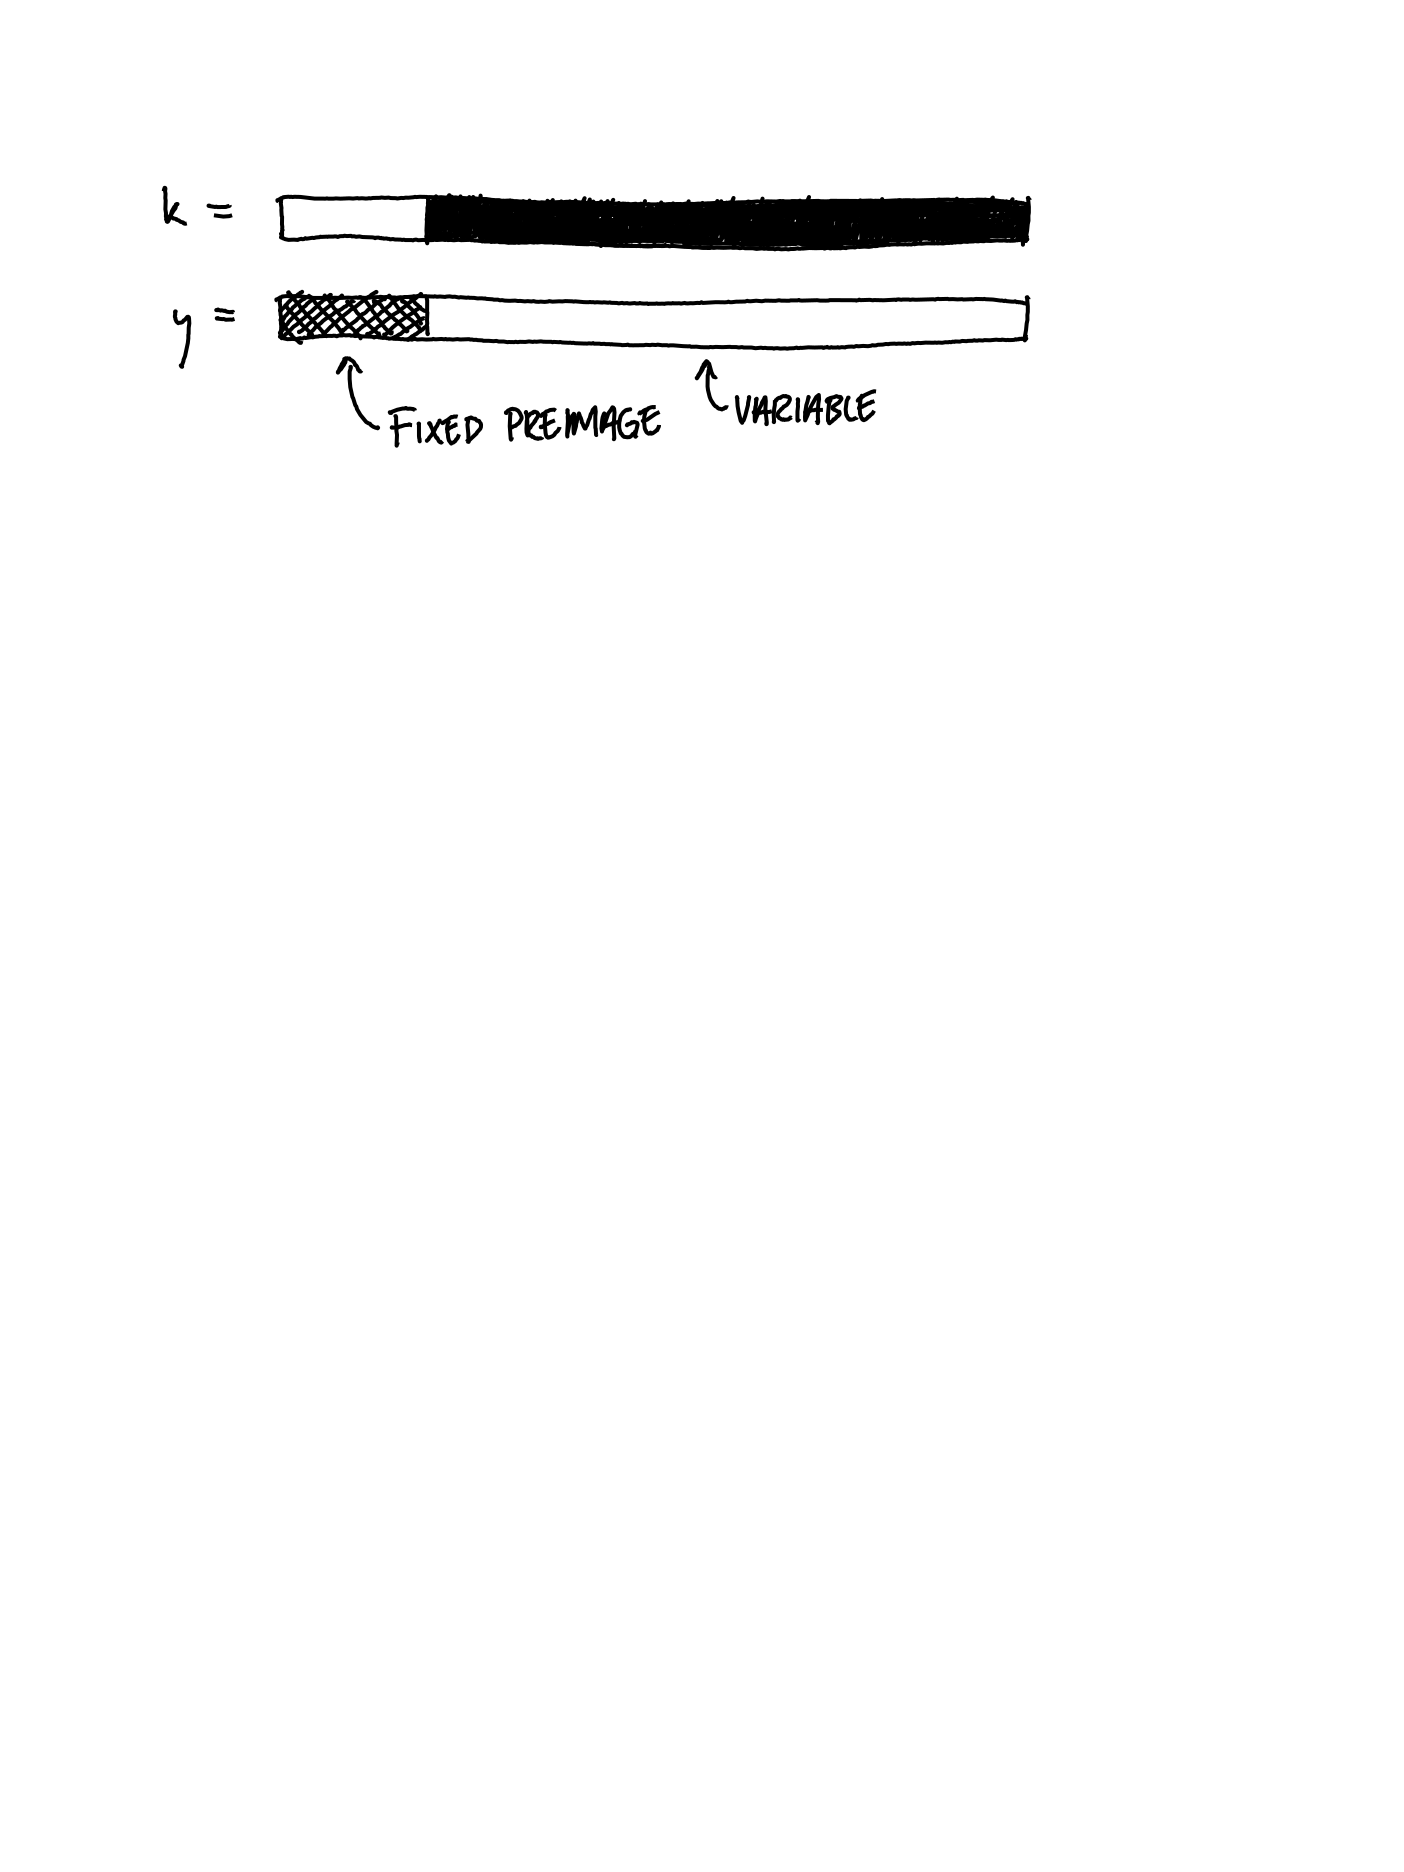
\includegraphics[width=0.8\columnwidth]{fig/pow.pdf}
    \caption{Proof-of-work problem}
  \end{figure}
\end{frame}

\begin{frame}
  \begin{figure}
    \centering
    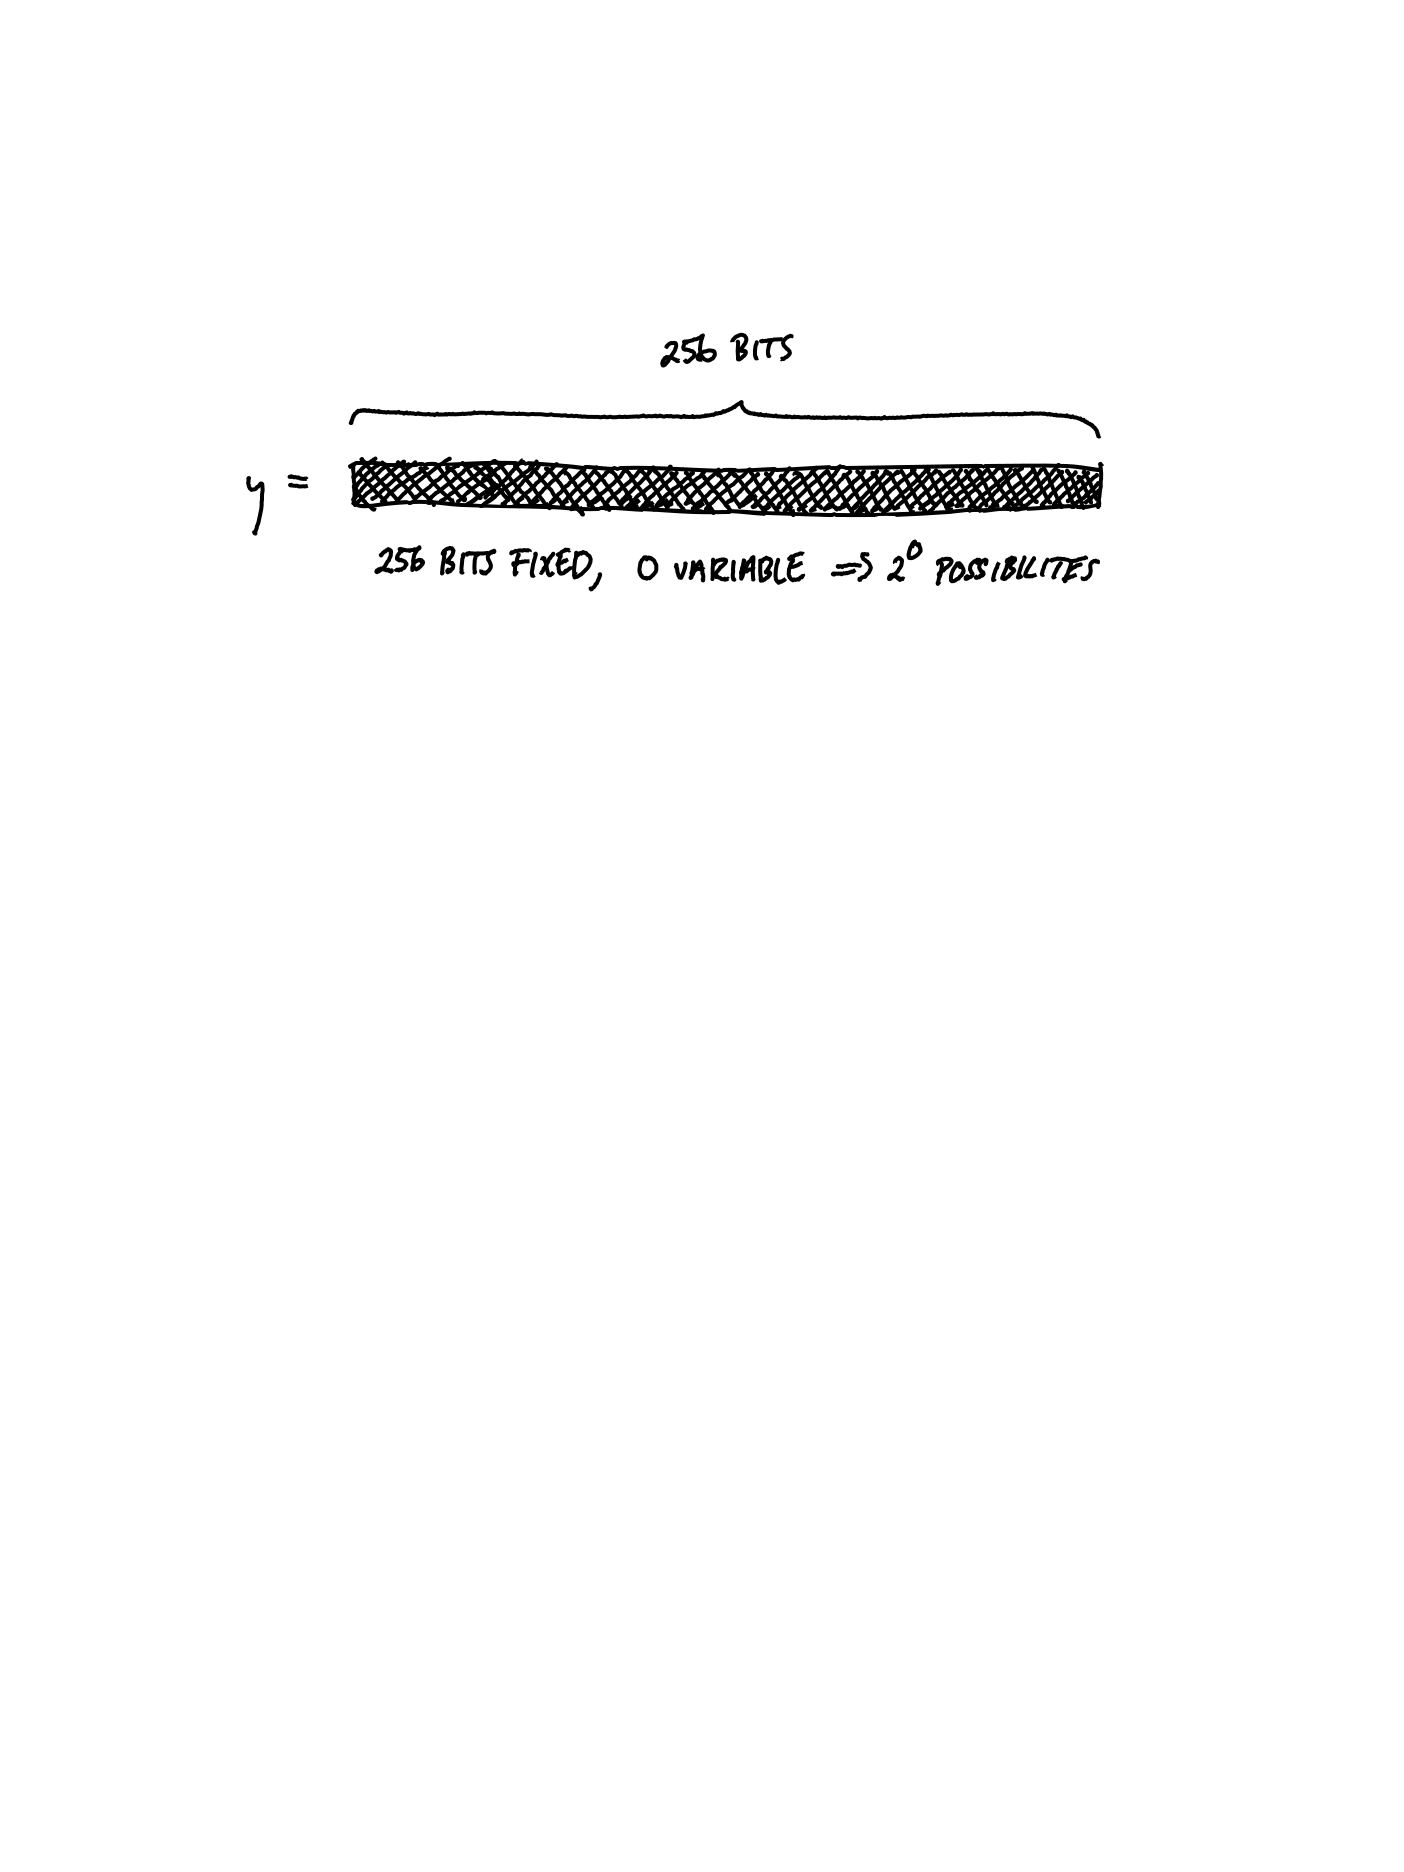
\includegraphics[width=0.8\columnwidth]{fig/preimage.pdf}
    \caption{Preimage problem}
  \end{figure}
\end{frame}

\section{Tree hashing}

\begin{frame}
  \begin{question}
    \only<presentation>{%
      \begin{itemize}
        \item If blocks contain many transactions, what do light clients do?
        \item How can you verify inclusion without downloading everything?
      \end{itemize}
    }
    \only<article>{%
      Hash chaining gives us an ordered history of blocks, but each block may
      contain many transactions. A natural next question is: how can a party
      verify that a particular transaction is included in a block without
      downloading (and rehashing) the entire set of transactions?
    }
  \end{question}
\end{frame}

\ltnote{%
  \textbf{Try-first}: Ask for a verification strategy before introducing Merkle
  trees.

  \textbf{Variation pattern}: Contrast between verifying \emph{everything} (the
  whole block) and verifying \emph{one item} (one transaction) with a short
  proof.

  \textbf{Critical aspects}: Hashing compresses a large set into a root hash, and
  a Merkle authentication path reveals only what is needed to verify inclusion.
}

\begin{frame}
  \begin{figure}
    \includegraphics[width=0.9\columnwidth]{fig/merkle-tree.png}
    \caption{Merkle tree}
  \end{figure}
\end{frame}

\begin{frame}
  \begin{figure}
    \includegraphics[width=\textwidth]{fig/bitcoin-powchain.png}
    \caption{Merkle trees for transactions.
      Only need Hash01, Hash2 to verify Tx3 is in there.
    Image:~\cite{Nakamoto2008bap}.}
  \end{figure}
\end{frame}

